\documentclass[11pt]{article}

\usepackage{fullpage}
\usepackage{amsfonts}
\usepackage{graphicx}

\def\eq1{y=\frac{x}{3x^2+x+1}}
\def\labelaxes{Remember to include a scale and label your axes.}

\begin{document}

The set of Natural numbers is denoted 
$\mathbb{N}$.

The set of Integers is denoted by 
$\mathbb{Z}$.

The set of Real numbers is denoted by 
$\mathbb{R}$.

Graph $\eq1$.\labelaxes

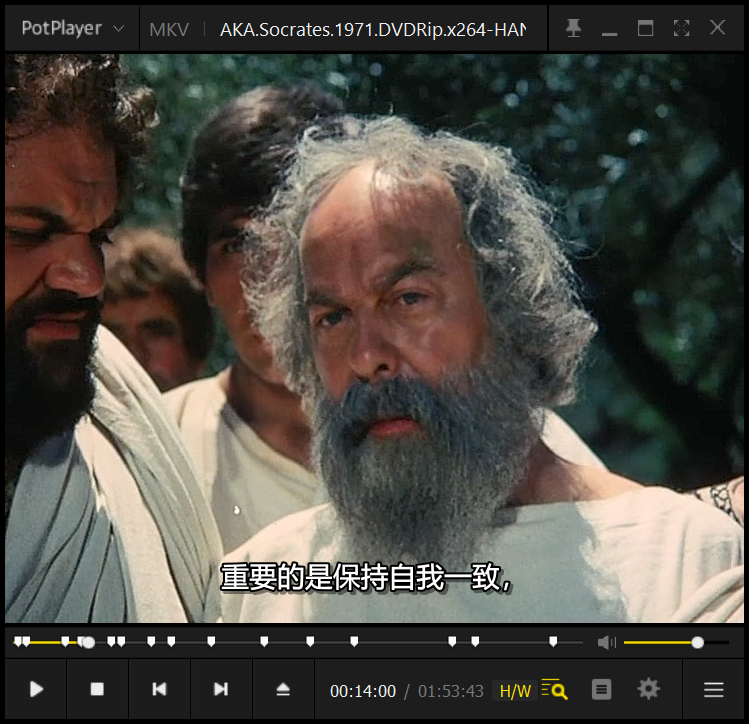
\includegraphics[scale=0.2, angle=45]{5.png}

Identify the asymptotes for the graph of
$\eq1$.

\end{document}